\section{Definition}

\subsection{Project Overview}

Object recognition is a major discipline in the field of computer vision. The applications are numerous and varied as self-driving vehicles environment detection, skin cancer screening or reality augmented tourism.


This project focus on the automatic recognition of flower species from pictures with potential applications such as:

\begin{itemize}
	\item population tracking and preservation (imagine drones taking a census of flowers in your neighborhood)
	\item crop and food supply management 
	\item toxicity detection 
	\item Education (i.e. smartphone app for hitch-hiker and nature lovers)
\end{itemize}

\begin{center}
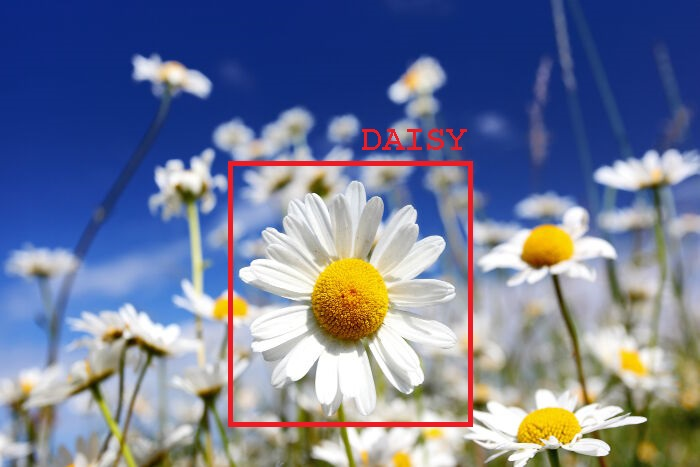
\includegraphics[scale=1.3]{Daisy_detection.jpg}
\captionof{figure}{it's a Daisy!}
\end{center}


\subsection{Problem Statement}

Is it possible to accurately identify the variety of a flower from a picture ?

The today state of the art solution to tackle pictures classification problems is the creation and training of a deep Convolution Neural Network (CNN). The training has to be performed on a dataset  of flower pictures classified by species. 

\subsection{Dataset}

The dataset used in this project is the \lq\lq{}Flowers Recognition Dataset\rq\rq{} of  \href{https://www.kaggle.com/alxmamaev/flowers-recognition}{Kaggle.com}  given by \href{https://alxmamaev.github.io/}{Alexander Mamaev}.\\

The zip archive is 230MB and contains about 4300 flower images (.jpg) classified in 5 classes: Daisy, Dandelion, Rose, Sunflower and Tulip.

\begin{center}
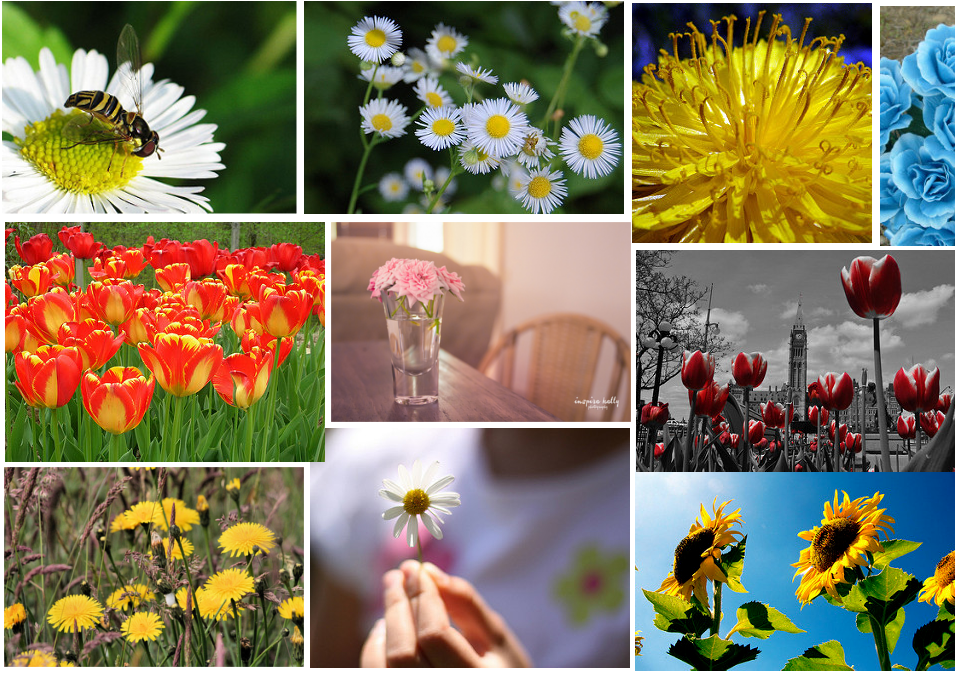
\includegraphics[scale=.2]{flowers_patchwork.png}
\captionof{figure}{samples of "Flowers Recognition" dataset}
\end{center}

The pictures appear to have been automatically scraped from the online picture portals Klickr, Google Images and Yandex Images.


The pictures represents single or multiple flowers under various angles, zoom, brightness conditions, life cycle stages. However, a significant number of pictures contains other subjects (persons, insects, other flowers, vase) or seem to be miss-classified. Such pictures can potentially negatively impact the training of the CNN. A more detailed approach of the selection of suitable samples is described in chapter \fullref{subsec:Data_Preprocessing} 


\subsection{metrics}

The evaluate our classification model is based on the \textit{Accuracy} $ACC$ and the \textit{Classification Cross-Entropy} $H(y, \hat{y})$ metrics defined as follows: 


\begin{center}

	$ACC = \frac{number \ of \ correct \ predictions}{total \ number \ of \ prediction} \cdot 100$ \\

\end{center}


\begin{center}
$H(y, \hat{y})=-\sum_{k=1} y_i log(\hat{y_i})$
\end{center}
	